%---------------------------------------------------
% کلاس سند: article برای اسناد متنی، با اندازه کاغذ A4 و فونت پایه 16
\documentclass[a4paper,16pt]{article}

% بسته‌های ریاضی برای معادلات و نمادهای پیشرفته
\usepackage{amsmath, amssymb, amstext}

% بسته رنگ برای استفاده از رنگ در متن یا محیط‌ها
\usepackage{xcolor}

% بسته گرافیک برای درج تصاویر
\usepackage{graphicx}

% تنظیمات حاشیه صفحه
\usepackage{geometry}

% بسته لینک‌دهی (هایپرلینک‌ها)
\usepackage{hyperref}

% بسته صفحه‌آرایی برای تنظیم هدر و فوتر
\usepackage{fancyhdr}


% بسته xepersian برای پشتیبانی از زبان فارسی با XeLaTeX
\usepackage{xepersian}

% تعیین فونت فارسی (فایل فونت باید موجود باشد یا در سیستم نصب باشد)
\settextfont{B Nazanin}

% تنظیم اندازه حاشیه‌ها از هر طرف برابر با 1 اینچ
\geometry{margin=1in}

% تنظیم سبک fancy برای سربرگ و پاورقی
\pagestyle{fancy}

% سمت چپ هدر: مشخص‌کننده سری تمرین و نام درس
\lhead{تمرین سری یک درس فیزیک\lr{II }}

% وسط هدر: نام دانشکده
\chead{دانشکده فیزیک دانشگاه صنعتی خواجه نصیرالدین طوسی}

% سمت راست هدر: تاریخ روز به‌صورت خودکار
\rhead{\today}

% پایین صفحه: شماره صفحه
\cfoot{\thepage}

% شروع سند
\begin{document}
	
	% صفحه عنوان (بدون هدر و فوتر)
	\thispagestyle{empty}
	\begin{center}
		% لوگوی دانشگاه (باید فایل تصویر در مسیر پروژه باشد)
		
		
\includegraphics[width=0.5\textwidth]{../../../images/image-E_1/image-1.png} \\[10pt] 
		% عنوان سند
		\textbf{\LARGE عنوان:تمرین سری‌یک}\\[20pt]
		
		% نیم‌سال تحصیلی
		\textbf{\LARGE نیم‌سال تحصیلی:4032 }\\[10pt]
		
		% نام مدرس درس
		\textbf{\Large مدرس: ‫دكتر‬ ‫رضا‬ ‫افضل‬ ‫زاده‬}\\[10pt]
		
		% مبحث تمرین 
		\textbf{\Large  مبحث تمرین:‫قانون‬ ‫كولن‪،‬‬ ‫ميدان‬ ‫الكتريكي‬  }\\[10pt]
		
		% مهلت تحویل تمرین
		\textbf{\Large مهلت تحویل:22 فروردین }
	\end{center}
	
	% صفحه جدید برای ادامه سند
	\newpage
	
	% ایجاد فهرست مطالب به‌صورت خودکار (براساس \section و \subsection و ...)
	\tableofcontents
	\newpage
	
	
	\section{سوال اول}
	ثابت کنید:در شکل زیر، چهار ذره یک مربع را تشکیل می‌دهند. بارهای الکتریکی به صورت زیر هستند:
	\[
	q_1 = 3q \qquad q_2 = 2q \qquad q_3 = 4q \qquad q_4 = q
	\]
	
	\begin{enumerate}
		\item[(الف)] نسبت $\dfrac{Q}{q}$ چقدر باید باشد تا نیروی الکترواستاتیکی خالص
		روی ذرات $1$ و $4$ صفر شود؟
		
		\item[(ب)] آیا مقداری برای $q$ وجود دارد که نیروی الکترواستاتیکی خالص
		روی هر چهار ذره صفر شود؟ توضیح دهید.
	\end{enumerate}
	\begin{center}
	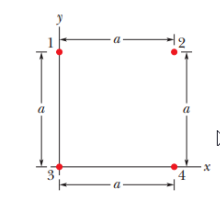
\includegraphics[width=0.5\textwidth]{../../../images/image-E_1/image-2.png} \\[10pt] 
	\end{center}

	\section{سوال دوم}
	ذره $1$ با بار $+1.0~\mu C$ و ذره $2$ با بار $-3.0~\mu C$ 
	در فاصله $L = 10.0~\mathrm{cm}$ روی محور $x$ قرار دارند.
	
	اگر ذره $3$ با بار نامعلوم $q_3$ در موقعیتی قرار گیرد که نیروی 
	الکترواستاتیکی خالص وارد بر آن از طرف ذرات $1$ و $2$ صفر شود،  
	مختصات $x$ و $y$ این ذره چه باید باشد؟
		\begin{center}
		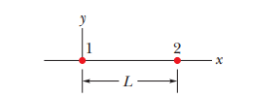
\includegraphics[width=0.5\textwidth]{../../../images/image-E_1/image-3.png} \\[10pt] 
	\end{center}
	
	\section{سوال سوم}
	دو ذره باردار در صفحه $xy$ ثابت نگه داشته شده‌اند. اطلاعات آن‌ها به شرح زیر است:
	\[
	\begin{aligned}
		q_1 &= +3.0~\mu C, \qquad &x_1 &= 3.5~\mathrm{cm}, \qquad &y_1 &= 0.50~\mathrm{cm}, \\
		q_2 &= -4.0~\mu C, \qquad &x_2 &= -2.0~\mathrm{cm}, \qquad &y_2 &= 1.5~\mathrm{cm}.
	\end{aligned}
	\]
	
	\begin{enumerate}
		\item[(الف)] اندازه نیروی الکترواستاتیکی وارد بر ذره $2$ از طرف ذره $1$ چقدر است؟
		
		\item[(ب)] جهت نیروی الکترواستاتیکی وارد بر ذره $2$ از طرف ذره $1$ چگونه است؟
		
		\item[(ج)] مختصات $x$ و $y$ برای قرار دادن ذره سوم با بار
		$q_3 = +4.0~\mu C$
		به‌گونه‌ای که نیروی الکترواستاتیکی خالص وارد بر ذره $2$
		از طرف ذرات $1$ و $3$ صفر شود، کجا باید باشد؟
	\end{enumerate}
	
	\section{سوال چهارم}
	در شكل زير، دو توپ ريز هادي با جرم يكسان $m$ و بار يكسان $q$
	از نخ هاي غيررسانا با طول $L$ اويزان هستند.
	فرض كنيد زاويه $\theta$ آن قدر كوچك است كه بتوان
	$\tan\theta$ را با تقريب برابر $\sin\theta$ در نظر گرفت.
	
	\begin{enumerate}
		\item[(الف)] نشان دهيد كه فاصله تعادلي $x$ بين دو توپ از رابطه
		\[
		x = \left( \frac{L q^2}{2\pi \varepsilon_0 m g} \right)^{1/3}
		\]
		به دست مي آيد.
		
		\item[(ب)] اگر
		\[
		L = 120~\mathrm{cm}, \qquad
		m = 10~\mathrm{g}, \qquad
		x = 5.0~\mathrm{cm}
		\]
		باشد، مقدار $|q|$ را محاسبه كنيد.
	\end{enumerate}
	\begin{center}
		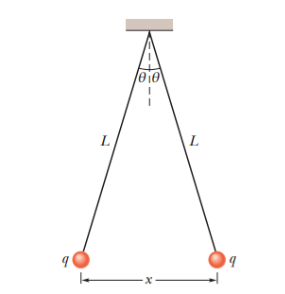
\includegraphics[width=0.5\textwidth]{../../../images/image-E_1/image-4.png} \\[10pt] 
	\end{center}
	\newpage
	\section{سوال پنجم}
	\begin{enumerate}
		\item[(الف)] ميدان الكتريكي در نقطه $P$ به ازاي يك حلقه باردار چگونه به دست مي آيد؟
		
		\item[(ب)] حالا فرض كنيد به جاي حلقه، يك قرص باردار داريم.
		ميدان الكتريكي در نقطه $P$ كه در نزديكي اين قرص قرار دارد، چگونه به دست مي آيد؟
	\end{enumerate}
	\begin{center}
		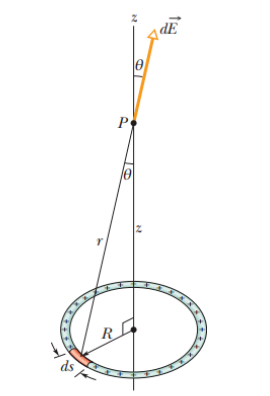
\includegraphics[width=0.5\textwidth]{../../../images/image-E_1/image-5.png} \\[10pt] 
	\end{center}
	\section{سوال ششم}
	يك حفره دلخواه درون يك جسم رسانا را در نظر بگيريد.
	اگر يك بار نقطه اي $q$ درون اين حفره قرار داشته باشد،
	نشان دهيد كه بار القا شده روي سطح داخلي حفره
	برابر با $-q$ خواهد بود.
	\section{سوال هفتم}
	‫با‬‫استفاده‬ ‫از‬ ‫قانون‬ ‫گاوس‬ ‫ميدان‬ ‫الكتريكي‬ ‫را‬ ‫براي‬ ‫يك‬ ‫خط‬ ‫بار‬ ‫بينهايت‬ ‫بدست‬ ‫بياوريد‬
	\section{سوال امتیازی}
	
	‫ميدان‬‫ الكتريكي‬ ‫را‬ ‫براي‬ ‫يك‬ ‫خط‬ ‫بار‬ ‫بينهايت‬ ‫بدست‬ ‫بياوريد(بدون‬ ‫استفاده‬ ‫از‬ ‫قانون‬ ‫گاوس)‬
	\\

	\textbf{موفق باشید.}
\end{document}
